\documentclass[12pt, letterpaper]{article}
\usepackage{graphicx} % Required for inserting images
\usepackage{hyperref}
\usepackage{xcolor}
\usepackage{amssymb}
\usepackage{amsmath}
\usepackage[english]{babel}
\usepackage{nicefrac, xfrac}
\usepackage{epsfig}
\newcommand{\Z}{{\mathbb Z}}
\newcommand{\R}{{\mathbb R}}
\newcommand{\N}{{\mathbb N}}
\newcommand{\E}{{\mathbb E}}
\newcommand{\V}{{\mathbb V}}
\newcommand{\acc}{\\\hphantom{}\\}
\newcommand{\Prob}{{\mathbb P}}
\usepackage[paper=a4paper,left=20mm,right=20mm,bottom=25mm,top=25mm]{geometry}
\title{Calcolo delle Probabilità}
\author{Marco Casu}
\date{\vspace{-5ex}}
\begin{document}



\maketitle
\begin{figure}[h]
    \centering{
    
\includegraphics[width=0.9\textwidth ]{images/cop.jpeg}
    }
\end{figure}
\newpage
\tableofcontents
\newpage
\section{Il Modello Probabilistico}
\subsection{Il Problema dei Compleanni}
Qaunte sono le probabilità che in un gruppo di 25 persone, 2 di queste siano nate lo stesso giorno? 
Procediamo nel \textbf{modellizzare} tale problema.
Le possibili date di nascita sono 365. 
\centering\(PossibiliDate=\{1,2,3,4...,365\}\)\\
\raggedright Intervistando un singolo individuo, questo può darmi 365 risposte, la probabilità che quindi
un individuo di nome \textit{Tizio} sia nato lo specifico giorno \(i\) è di 1 su 365.\\
\centering\( \mathbb{P}(\text{\textit{Tizio} è nato il giorno } i) = \dfrac{1}{365} \)\\
\raggedright Tale probabilità si dice \textbf{uniforme} perchè tutti i 365 esiti hanno la stessa
probabilità di \(\frac{1}{365}\) di risultare.
Adesso, quante sono le probabilità che \textit{Tizio} sia nato il giorno \(i\) e \textit{Caio}
il giorno \(j\)?\\
\centering\( \mathbb{P}(\text{\textit{Tizio} è nato } i \text{ e \textit{Caio} è nato } j) = \mathbb{P}(\text{\textit{Tizio} è nato il giorno } i) \cdot \mathbb{P}(\text{\textit{Caio} è nato il giorno } j) \)\\
\raggedright Questo si chiama \textbf{concetto di indipendenza}, ed è ovvio che le probabilità sono precisamente \(\dfrac{1}{365}\cdot\dfrac{1}{365} = \bigg( \dfrac{1}{365}\bigg)^2 \).
Quindie probabilità che 25 persone siano nate in 25 giorni pre determinati sono precisamente : \\
\centering\( \mathbb{P}( a_1 \text{ è nato } i_1,a_2 \text{ è nato } i_2...,a_{25} \text{ è nato } i_{25}) = \bigg( \dfrac{1}{365}\bigg)^{25} \)\\
\raggedright
Queste sono le probabilità che 25 persone siano nate lo stesso giorno, a noi ci interessano però
le probabilità che almeno 2 persone siano nate lo stesso giorno. Prima di fare ciò andiamo a definire
quello che si dice \textbf{modello probabilistico}.\\
Chiamiamo \(\Omega\) lo spazio degli eventi elementare (in seguito verrà definito in modo formale), 
Ossia l'insieme di tutti i possibili risultati dell'esperimento. Sia l'esperimento in questo caso, la 
data di nascita per \(k\) persone, il nostro \(\Omega\)  sarà l'insieme di tutte le possibili combinazioni 
lunghe 25 di  numeri da 1 a 365, che sono precisamente \(|\Omega|=365^{25}\). La probabilità uniforme
che un certo evento dello spazio degli eventi \(\Omega={\omega_1,\omega_2...,\omega_k }\) accada è \(\mathbb{P}({\omega_i})=\dfrac{1}{|\Omega|}\).
Definiamo adesso un evento \textbf{binario}, ossia un evento che ha come risposta, o si o no,ossia le probabilità che 
esso accada e che esso non accada. Definiamo l'evento \(A\) come l'evento in cui almeno 2 persone fanno il compleanno
lo stesso giorno.\\
\centering\( A=\{\omega \in \Omega :\exists \omega_i,\omega_j \in \omega | i\ne j \land \omega_i=\omega_j\} \)\\
\raggedright
Quindi tale \(A\) è un sotto-insieme di \(\Omega\) in cui tutti gli elementi hanno almeno 2 date uguali. 
Presa con \(|A|\) la cardinalità di tale sotto-insieme, le probabilità che tale evento accada sono :\\
\centering\( \mathbb{P}(A)=\dfrac{|A|}{|\Omega|} \)\\
\raggedright Piuttosto che trovare l'evento in cui ci sono almeno 2 persone con lo stesso  compleanno,
è più facile trovare il suo \textbf{complementare}, ossia l'evento in cui nessuno fa il compleanno lo stesso giorno.
\\\centering\( A^c=\{\omega \in \Omega | \forall i\ne j, \omega_i \ne \omega_j\} \)\\
\raggedright Una volta trovata la probabilità di \(A^c\), sapremo che \(\mathbb{P}(A)=1-\mathbb{P}(A^c)\).
\\\centering essendo \(k=25 \) e \( n=365 \rightarrow |A^c|=n \cdot (n-1) \cdot (n-2)...\cdot (n-k+1)  \implies
 \mathbb{P} (A)=1-\dfrac{|A^c|}{365^{25}}\)  \\
\raggedright Vediamo una tabella di possibili risultati al variare di \(k\) (numero di persone) :\\\hphantom{.}\\
\centering
    \begin{tabular}{|l|l|l|l|l|l|}
    \hline
    \(k\)  & 4    & 16   & 22   & 23   & 63   \\ \hline
    \(\mathbb{P}(A)\) & 0.06 & 0.28 & 0.42 & 0.50 & 0.99 \\ \hline
    \end{tabular}
\\\raggedright
 Risulta chiaro come, intervistando 25 persone, c'è una probabilità superiore 
al 50 \% che almeno due di esse condividano il compleanno.
\subsection{Assiomi della probabilità}
Definiamo adesso formalmente il \textbf{modello probabilistico}, esso ha 3 ingredienti :
\\\hphantom{.}\\\textbf{1 - Lo Spazio degli Eventi Elementari}

Detto anche \textit{spazio campionario}, non è altro che l'insieme di tutti i possibili esiti dell'
esperimento, e viene denominato con \(\Omega\). Ad esempio, se l'esperimento è il lancio di una moneta,
si avrà \(\Omega=\{\)Testa,Croce\(\}\). Nel caso dell'esperimento dei compleanni, lo spazio campionario 
sarà composto da tutte le possibili combinazioni lunghe \(k\) ( numero di persone alla quale si chiede 
la data di nascita ) di numeri da 1 a 365 (i giorni esistenti). Per la maggior parte dei casi analizzati 
in questo corso, \(\Omega\) sarà un insieme finito. Si indica con \(|\Omega|\) la cardinalità dello 
spazio campionario, ossia il numero dei suoi elementi.
\\\hphantom{.}\\\textbf{2 - Algebra degli Eventi}

Prima di definire l'algebra degli eventi, dichiariamo cos'è un \textbf{evento}, ossia una \textit{domanda
binaria} sull'esito dell'esperimento, in termini matematici, è un qualsiasi sotto-insieme \(\Omega\), compresi
gli elementi singoli di \(\Omega\), detti \textbf{eventi elementari}. Se l'esperimento è il lancio di un dato,
i possibili esiti sono \(\Omega=\{1,2,3,4,5,6\}\), vogliamo definire l'evento \(A\) come la probabilità
che l'esito del lancio sia un numero maggiore di 4, esso non è altro che un sotto-insieme dello spazio campionario,
ossia \(A=\{\omega \in \Omega | \omega \ge 4 \}=\{4,5,6\}\). 

Su tali eventi sono definite delle operazioni insiemistiche di unione, intersezione e complemento.\\
L'Algebra degli Eventi, definita con il simbolo \(\mathcal{A} \), è l'insieme chiuso\footnote{
    È un insieme chiuso rispetto alle operazioni di unione, intersezione e complemento, ossia il risultato
    di tali operazioni su uno o più elementi dell'insieme, è sempre parte di tale insieme.
    } 
 di \textit{tutti
i possibili sotto-insiemi} dello spazio campionario, ossia tutti i possibili eventi 
(anche non elementari) per la quale si può misurare la probabilità. 
\textit{Ad esempio}, se prendiamo il caso del dado \(\Omega=\{1,2,3,4,5,6\}\), l'evento
in cui il risultato sia 2 o 3, è l'unione dei due eventi elementari \(A=\{2\}\) e \( B=\{3\} \rightarrow C = A \cup B
= \{2,3\}\). Si noti che \(|\Omega|=n \implies |\mathcal{A}|=2^n\)
\\\hphantom{.}\\\textbf{3 - La Funzione Probabilità}
La probabilità di un determinato evento appartenente ad \(\mathcal{A} \) è misurata tramite una 
funzione definita come \(\mathbb{P} : \mathcal{A} \rightarrow [0,1]\), essa associa ad ogni elemento
dell'algebra degli eventi, una probabilità misurata tra 0 ed 1, dove 0 indica che l'evento è impossibile,
ed 1 che l'evento è certo. La funzione \(\mathbb{P}\) deve soddisfare 3 condizioni :
\begin{itemize}
    \item \(\mathbb{P}(\emptyset )= 0\) La probabilità dell'insieme vuoto è 0.
    \item \(\mathbb{P}(\Omega)= 1\) La probabilità che si verifichi un evento di \(\Omega\) è l'evento certo.
    \item \(\mathbb{P}\) è una funzione \textit{additiva}, ossia che per due eventi disgiunti \(A\) e 
    \(B\), nel senso che \(A\cap B = \emptyset\), vale che \(\mathbb{P}(A\cup B)=\mathbb{P}(A)+\mathbb{P}(B)\).
\end{itemize}
Vediamo adesso \textbf{alcune considerazioni} riguardo gli assiomi appena enunciati.\\
Risulta ovvio che \(\Omega = A\cup A^c \implies \mathbb{P}(A^c)=1-\mathbb{P}(A)\). Diversamente, presi 
due eventi \(A\) e \(B\) \textit{non necessariamente disgiunti}, vale che \(\mathbb{P}(A\cup B)
=\mathbb{P}(A)+\mathbb{P}(B)-\mathbb{P}(A\cap B)\). Un'altra considerazione, è che \(\mathbb{P}\)
 è una funzione \textit{monotona} rispetto all'inclusione di insiemi, detto formalmente 
 \(A \subseteq B \implies \mathbb{P}(A) \le \mathbb{P}(B)\).
\\ Quando si vuole misurare la probabilità di un evento in un certo 
esperimento, bisogna quindi costruire un modello probabilistico, definendone gli eventi elementari e
 la probabilità ad essi associati. Possiamo quindi definire un altra funzione \(p\), che ha come dominio
 esclusivamente gli eventi elementari \(\Omega\), e non gli eventi di \(\mathcal{A}\), essa sarà 
 denominata come \textbf{probabilità degli eventi elementari}, \(p:\Omega \rightarrow [0,1]\). Risulta
 chiaro che \(\displaystyle\sum_{\omega \in \Omega} p(\omega)=1  \).\\
 Ad esempio, facciamo un esperimento sul lancio di un dado truccato in cui è più probabile che esca 
 il numero 6 piuttosto che altri :
 \\ \center \(\Omega=\{1,2,3,4,5,6\}\)\\
 \raggedright\( p(1)=p(2)=p(3)=0.1\)\\\( p(4)=p(5)=0.2\)\\\(p(6)=0.3\)
 \\
 Definiamo quindi \(\displaystyle\mathbb{P}(A)=\sum_{\omega \in A}p(\omega)\), e risulta chiaro che :\\
 \centering
 \(\displaystyle\sum_{\omega \in \Omega}p(\omega)=\sum_{\omega \in A}\mathbb{P} (\{\omega\})=
 \mathbb{P}(\bigcup_{\omega \in \Omega}\{\omega\} )=1\)
 \\\raggedright La probabilità in un modello probabilistico, si dice \textbf{uniforme} se \(p(w)=\dfrac{1}{|\Omega|} \) \(\forall \omega \in \Omega\)
, e significa che tutti gli eventi elementari hanno la stessa probabilità di accadere, da qui ne deriva che la 
probabilità di un evento \(A\in \mathcal{A} \) è \(\mathbb{P}(A)=\dfrac{|A|}{|\Omega|}\).
\section{Calcolo Combinatorio}
Riassumiamo in questa sezione ciò che si è visto nel corso di \textit{Metodi matematici per l'informatica}. Partiamo
con un problema, si dia il caso che in un urna ci sono 3 palline bianche e 2 palline nere, qual'è la probabilità che, 
estraendo due palline, la seconda sia bianca? Formalizziamo il problema secondo il modello probabilistico.
L'evento elementare è l'estrazione \textit{ordinata} di due palline \(\omega=(\omega_1,\omega_2)\), dove 
\(\omega_1\) = prima estratta e \(\omega_2\) = seconda estratta. Possiamo numerare le palline da 1 a 5, 
dicendo che le palline bianche son quelle da 1 a 3, e le restanti le nere. Detto ciò, possiamo capire che l'insieme 
degli eventi elementari, sono tutte le coppie di numeri naturali compresi fra 1 a 5 senza ripetizioni.
\begin{equation}
    \Omega = \{(w_1,w_2) | w_1,w_2 \in \{1,2,3,4,5\}, w_1 \ne w_2\}
\end{equation}
È di facile intuizione capire che \(|\Omega|=20\).\\
L'evento \(A\) invece rappresenta il sotto-insieme di \(\Omega\), dove 1,2 o 3 appaiano sempre come seconda 
coordinata dei suoi elementi, ossia tutte le estrazioni in cui la seconda pallina è bianca. Per calcolare \(\mathbb{P}(A)\),
dobbiamo capire qual'è prima la cardinalità di \(A\), che risulta essere \(|A|=3\cdot 4 = 12\), il 3 rappresenta 
le 3 possibili palline bianche della seconda estrazione, il 4 invece tutte le altre possibili rimanenti (per
 la quale non ci interessa il colore essendo la prima estrazione.) Fatto ciò si ha \(\mathbb{P}(A)=\dfrac{|A|}{|\Omega|}=\dfrac{12}{20}=\dfrac{3}{5}=0.6\). La 
 probabilità è quindi del 60\%.
 \subsection{Principio fondamentale del calcolo combinatorio}
 Dati due insiemi finiti e non vuoti \(A\) e \(B\), è possibile formare \(|A|\cdot|B|\) diverse coppie ordinate 
 prendendo un primo elemento da \(A\) ed un secondo elemento \(B\).
 \begin{equation}
    |A\times B|=|A|\cdot|B|
 \end{equation}
 \newpage Vediamo un \textit{esempio} :\\
 Lanciamo un dado 6 volte, quant'è la probabilità che esca almeno una delle volte 6? Diciamo che un evento 
 elementare \(\omega\) è una ennupla di 6 elementi (i lanci) composta da numeri da 1 a 6 (esiti del dado). 
 \begin{equation}
    \Omega = \{(\omega_1,\omega_2,...\omega_6) | \omega_i \in \{1,2,3,4,5,6\}\}
 \end{equation}
 Risulta chiaro (per il principio moltiplicativo) che \(|\Omega|=6^6\).
 Dobbiamo adesso calcolare la cardinalità di \(A=\{\omega \in \Omega | \exists \omega_i \in \omega \rightarrow\omega_i = 6\}\),
 ossia tutti gli eventi elementari in cui 6 compare almeno in un lancio. Ci risulta però più facile calcolare il 
 suo complementare, ossia tutti gli eventi in cui 6 non compare mai, ossia
 ogni ennupla di 6 elementi (i lanci) composta da numeri da 1 a 5 (esiti del dado escluso il 6). 
 \begin{equation}
    A^c = \{(\omega_1,\omega_2,...\omega_6) | \omega_i \in \{1,2,3,4,5\}\}
 \end{equation}
 Risulta chiaro (per il principio moltiplicativo) che \(|A^c|=5^6\).
 Avendo la \(|A^c|\), possiamo trovare la probabilità dell'evento \(A\) : 
 \begin{equation}
    \mathbb{P}(A)=1-\mathbb{P}(A^c)=1-\dfrac{|A^c|}{|\Omega|}=1-\dfrac{5^6}{6^6}\simeq 0.66
 \end{equation}
 \subsection{Modelli del calcolo combinatorio}
 Prima di parlare dei modelli del calcolo combinatorio, introduciamo un concetto importante :
 \begin{quote}
    \textbf{Permutazione}\\
    Sia \(S\) un insieme finito e non vuoto, una \textit{permutazione} di \(S\) è 
    una scelta di ordine tra gli elementi di \(S\). Le possibili permutazioni risultano essere \(|S|!\) .
 \end{quote}
 Passiamo adesso alla presentazione di alcuni modelli fondamentali nella quale spesso ricadono i problemi 
 di conteggio. I problemi verranno \textit{metaforizzati} secondo il problema delle palline nelle urne.
 \subsubsection{Caso 1 - Estrazioni Ordinate con Rimpiazzo}
Si hanno \(n\) palline dentro un urna e si vogliono fare \(k\) estrazioni con rimpiazzo, ossia, una volta
pescata una pallina, si reinserisce nell'urna (un elemento stesso può essere estratto più volte). Si tiene 
conto dell'ordine, quindi \(\{1,2,3\}\ne\{1,3,2\}\). Per problemi di questo tipo, vale che : 
\begin{equation}
    \Omega = \{(\omega_1,\omega_2...,\omega_k) | \omega_i \in \{1,2,3...,n\}\} \implies |\Omega|= n^k
\end{equation}
\subsubsection{Caso 2 - Estrazioni Ordinate senza Rimpiazzo}
Si hanno \(n\) palline dentro un urna e si vogliono fare \(k\) estrazioni senza rimpiazzo, ossia, una volta
pescata una pallina, essa non potrà essere ripescata (gli elementi di ogni estrazione sono distinti). Si tiene 
conto dell'ordine, quindi \(\{1,2,3\}\ne\{1,3,2\}\). Per problemi di questo tipo, vale che : 
\begin{equation}
    \Omega = \{(\omega_1,\omega_2...,\omega_k) | \omega_i \in \{1,2,3...,n\}|i\ne j \implies w_i\ne w_j\} \implies |\Omega|= \dfrac{n!}{(n-k)!}
\end{equation}
\textit{Esempio :}\\
7 persone si trovano in un ascensore dentro un palazzo di 10 piani e si apprestano a scendere su un piano,
quante sono le probabilità per cui tutte quante scendano su piani diversi? L'Evento elementare è 
composta da una ennupla di 7 elementi (le persone) composta da numeri che vanno da 1 a 10 (il piano in cui scendono).
Quindi : \\\begin{center} \(\Omega = \{(\omega_1,\omega_2...,\omega_7)|\omega_i = \{1,2,3,4,5,6,7,8,9,10\}\}\)
\end{center}
Dati i modelli precedenti risulta chiaro che \(|\Omega|=10^7\) e \(A=\{\)Ognuno scende su un piano diverso\(\}\) ha cardinalità
 \(|A|=\dfrac{10!}{3!}\implies \mathbb{P}(A)=\dfrac{\frac{10!}{3!}}{10^7}\simeq0.06\) .
 \subsubsection{Caso 3 - Estrazioni non Ordinate senza Rimpiazzo}
 Si hanno \(n\) palline dentro un urna, se ne estraggono \(k\), ma senza tener conto dell'ordine delle palline, ad esempio,
 se ho le palline denominate 1,2 e 3, estraendole, si ha che le estrazioni 123, 321 ,132, 312, 231, 213 sono 
 lo stesso evento. Come rappresento tale spazio elementare \(\Omega\) a livello insiemistico? Si consideri lo spazio 
 delle \textit{Estrazioni Ordinate senza Rimpiazzo}, ossia:\begin{center} \( A  =\{(\omega_1,\omega_2...,
    \omega_k) | \omega_i \in \{1,2,3...,n\}|i\ne j \implies w_i\ne w_j\}\) \end{center}
Stabiliamo una relazione di equivalenza su \(A\), denominata con il simbolo \(\sim \), per cui 
vale che \(\omega\sim \omega'\) se e solo se differiscono solo per l'ordine. \\\textit{Esempio :}
\(\omega=\{1,2,3\},\omega'=\{3,1,2\}\iff \omega\sim \omega'\).
L'insieme degli eventi elementari per rappresentare le \textit{Estrazioni non Ordinate senza Rimpiazzo}
non è altro che l'insieme quoziente di \(A\) su \(\sim\), ossia l'insieme di tutte le sue classi di 
equivalenza.\begin{center}
    \(\displaystyle\Omega=\displaystyle\sfrac A\sim\)
\end{center}
Possiamo scegliere come rappresentanti delle classi di equivalenza, quegli elementi in cui le palline 
sono ordinate in ordine crescente, in tal modo, lo spazio elementare è anche rappresentabile come :
\begin{center}
    \(
        \{(\omega_1,\omega_2...,\omega_k)|\omega_i \in \{1,2,3...,n\} \land i<j\implies w_i < w_j\}
    \)
\end{center}
Qual'è però la cardinalità di \(\Omega\) in questo caso? Possiamo considerare la cardinalità di \(A\), divisa 
per il numero di elementi in ogni classe di equivalenza. Essendo che ogni classe di equivalenza non è altro
permutazione di \(k\) elementi, esse avranno ognuna \(k!\) elementi, da qui risulta chiara la cardinalità del 
nostro spazio degli eventi :
\begin{equation}
    \text{sia } [\omega]\in \sfrac{A}{\sim} \text{,  si ha  } |\Omega|=\dfrac{|A|}{|[\omega]|}=\dfrac{n!}{k!\cdot(n-k)!} \text{ si denota come }\binom{n}{k} 
\end{equation}
Tradotto in linguaggio umano, \(\binom{n}{k}\) indica il numero di modi di scegliere \(k\) elementi da un insieme \(n\). Tale
conteggio è anche detto \textbf{combinazione semplice}.
Vale la proprietà : \begin{center}
    \(\displaystyle\binom{n+1}{k+1}=\binom{n}{k+1}+\binom{n}{k}\)
\end{center}
\large \textbf{Binomio di Newton}\\\begin{center}
\normalsize Siano \(a,b \in \mathbb{R}\) e \(n\in\mathbb{N}\), vale che \(
    \displaystyle(a+b)^n = \sum_{k=0}^{n}\binom{n}{k}\cdot a^{n-k}\cdot b
\)\end{center}
\subsubsection{Caso 4 - Estrazioni non Ordinate con Rimpiazzo}
\normalsize Consideriamo il lancio di 2 dadi identici, senza considerare l'ordine. Abbiamo che l'evento elementare 
è la coppia di numeri da 1 a 6 (senza contare l'ordine, quindi consideriamo la classe di equivalenza 
in cui i due dadi hanno esito in ordine crescente), lo spazio risulta quindi : \(\Omega=\{(\omega_1,\omega_2)|1\le\omega_1\le\omega_2\le 6\}\)
\\Se i due dadi fossero distinti e l'ordine avesse importanza, i possibili eventi sarebbero \(6^2\), ma in questo caso, 
non risulta la scelta naturale, dato che gli eventi \((a,b)\) e \((b,a)\) sono identici.\\\hphantom{.}\\ È il caso di un \textit{estrazione
non ordinata con rimpiazzo}, dato che estraggo due palline, senza contare l'ordine, con la possibilità di poter 
estrarre due volte la stessa pallina.\\
Se ho \(n\) palline e faccio \(k\) estrazioni, il numero di estrazioni possibili non ordinate con rimpiazzo 
risulta essere : \begin{equation}
    \binom{n+k-1}{k}
\end{equation}
Tornando al problema dei dadi, i possibili esiti sono : \begin{center}
    \(
        \displaystyle\binom{6+2-1}{2}=\dfrac{(6+2-1)!}{2!(6+2-1-2)!}=\dfrac{7!}{2!5!}=\dfrac{7\cdot6\cdot5\cdot4\cdot3\cdot2}{5\cdot4\cdot3\cdot2\cdot2}=\dfrac{7\cdot6}{2}=21
    \)
\end{center}
\subsection{Principio di Esclusione/Inclusione}
Siano \(A,B,C\subset \Omega\) tre eventi non necessariamente disgiunti di uno spazio di probabilità, se volessi 
calcolare la probabilità di \(A\cup B\), dovrei fare la somma delle probabilità di \(A\) e \(B\), sottraendo la 
probabilità dell'intersezione. Già con 3 eventi, se volessi la probabilità dovrei fare :
\begin{center}
    \(\mathbb{P}(A\cup B\cup C)=\mathbb{P}(A)+\mathbb{P}(B)+\mathbb{P}(C)-(\mathbb{P}(A\cap B)+\mathbb{P}(A\cap C)+\mathbb{P}(B\cap C))+\mathbb{P}(A\cap B \cap C)\)
\end{center}
Quando si parla quindi di un numero elevato di eventi, il calcolo risulta difficile, ed è descritto dalla seguente formula :
\begin{equation}
    \mathbb{P}(A_1\cup A_2...,\cup A_n)=\sum_{k=1}^n(-1)^{k+1}\cdot\sum_{1<i_1<i_2...,<i_k<n}\mathbb{P}(A_{i_1}\cap A_{i_2}...,\cap A_{i_k})
\end{equation}
\subsection{Il Multinomio}
Esaminiamo il problema in cui si vogliono distribuire \(n\) oggetti distinti in \(k\) scatole distinte, in modo che 
ciascuna di esse contenga nell'ordine \(n_1,n_2...,n_k\) oggetti, per cui \(\displaystyle\sum_{i=1}^n n_i =n\). In quanti modi posso 
effettuare tale suddivisione? Ci sono \(\binom{n}{n_1}\) scelte per la prima scatole, \(\binom{n-n_1}{n_2}\) per la seconda 
e così via, fino a \(\dfrac{n!}{n_1!\cdot n_2!...,\cdot n_k!}\), che si denota con \(\displaystyle\binom{n}{n_1,n_2...,n_k}\), e 
rappresenta il numero di suddivisioni di \(n\) oggetti distinti in \(k\) gruppi distinti con, rispettivamente
\(n_1,n_2...,n_k\) oggetti.\\
\hphantom{.}\\\textit{Esempio : }Vi sono 10 poliziotti, se 5 di essi devono pattugliare due strade, 2 di essi 
restare in stazione ed altri 3 stare in riserva, quanti sono i modi possibili di assegnare i 3 compiti ai 
10 poliziotti? \begin{center}
    \(
      \displaystyle\binom{10}{5,2,3}=\dfrac{10!}{5!\cdot2!\cdot3!}=\dfrac{10\cdot9\cdot8\cdot7\cdot6\cdot5\cdot4\cdot3\cdot2}{5\cdot4\cdot3\cdot2\cdot 3 \cdot 2 \cdot 2}=\dfrac{30240}{12}=2520  
    \)
\end{center}
\subsection{Problema degli Accoppiamenti}
Poniamo un esempio, c'è una festa con \(n\) invitati, ogni invitato porta con se un ombrello, 
al termine della festa ogni invitato se ne va prendendo un ombrello a caso, qual'è la probabilità 
che nessun invitato riprenda il proprio ombrello? Se il numero di persone \(n\) tende ad 
infinito, come si comporta tale probabilità?\\\hphantom{.}\\ Si dice che in uno spazio di probabilità, 
se un evento elementare composto da una lista \(a_1,a_2...,a_n\) che possono assumere 
valori da \(1\) ad \(n\), se un elemento \(a_i\) assume valore \(i\), esso si dice \textbf{punto fisso},
quindi possiamo tradurre il problema degli ombrelli (considerando ogni persona come un elemento dell'evento 
elementare, ed i valori che possono assumere come gli ombrelli) come : Qual'è la probabilità che una permutazione 
di \(n\) non abbia punti fissi?\begin{center}
    \(\Omega=\{(\omega_1,\omega_2...,\omega_n)|i\ne j \implies \omega_i\ne \omega_j |\omega_k \in \{1,2,3...,n\} \}\) dove \(|\Omega|=n!\)
    \\\(B=\{\)permutazioni senza punti fissi\(\}=\{\omega\in\Omega | \forall i \in\{1,2,3...,n\} \omega_i\ne i \}\)
\end{center}
Poniamo il complementare di \(B\), ossia \(B^c=A=\{\)la permutazione ha almeno un punto fisso\(\}\), e distinguiamolo 
in \(n\) sotto eventi, ossia \(A_1=\{\omega_1\) è un punto fisso\(\}\) poi 
\(A_2=\{\omega_2\) è un punto fisso\(\}\) e così via per ogni punto. Sapremo così che 
\(A=A_1\cup A_2..., \cup A_n\). Calcoliamo la cardinalità di un singolo evento \(A_i\), risulta 
facile, dato che poniamo un punto fisso su \(\omega_i = i\) e poi il resto è una permutazione 
normale. \(|A_i|=(n-1)!\), quindi \(\mathbb{P}(A_i)=\dfrac{(n-1)!}{n!}=\dfrac{1}{n}\). Quindi per calcolare 
la probabilità di \(A\) dobbiamo sommare le probabilità di ogni \(A_i\), ma ovviamente tali sotto-eventi 
\textit{non sono disgiunti}, quindi dobbiamo sottrarre le intersezioni.
Notiamo come \(|A_i\cap A_j|=(n-2)!\), perchè fissiamo entrambi i punti \(i,j\) e ed il resto 
è una semplice permutazione. Questo fino a \(k\) intersezioni : \(|A_1\cap A_2...,\cap A_k|=(n-k)!\). Quindi :
\(\mathbb{P}(A_1\cap A_2...,\cap A_k) =\dfrac{(n-k)!}{n!}\). A questo punto applichiamo qui il 
\textbf{principio di esclusione/inclusione} :\begin{equation}
    \mathbb{P}(\bigcup^n_{k=1}A_k )=\sum_{i=1}^n (-1)^{k+1}\sum_{1<i_1<i_2...,<i_k<n}\mathbb{P}(A_1\cap A_2...,\cap A_k)
\end{equation}
Ma sappiamo che \(\mathbb{P}(A_1\cap A_2...,\cap A_k) =\dfrac{(n-k)!}{n!}\) quindi riscriviamo :\begin{equation}
    \mathbb{P}(\bigcup^n_{k=1}A_k )=\sum_{i=1}^n (-1)^{k+1}\sum_{1<i_1<i_2...,<i_k<n}\dfrac{(n-k)!}{n!}
\end{equation}
\begin{equation}
    \mathbb{P}(\bigcup^n_{k=1}A_k )=\sum_{i=1}^n (-1)^{k+1}\binom{n}{k} \dfrac{(n-k)!}{n!}
\end{equation}
\begin{equation}
    \mathbb{P}(\bigcup^n_{k=1}A_k )=\sum_{i=1}^n (-1)^{k+1}\dfrac{n!}{(n-k)!k!} \dfrac{(n-k)!}{n!}
\end{equation}
\begin{equation}
    \mathbb{P}(\bigcup^n_{k=1}A_k )=\sum_{i=1}^n (-1)^{k+1}\dfrac{1}{k!}
\end{equation}
Essendo \(A\) il complementare di \(B\) :
\begin{equation}
    \mathbb{P}(B)=1-\sum_{i=1}^n (-1)^{k+1}\dfrac{1}{k!}
\end{equation}
Con \(n\) che tende ad infinito si ha :
\begin{equation}
    \lim_{n\rightarrow \infty }\mathbb{P}(B)=1-\sum_{i=1}^n (-1)^{k}\dfrac{1}{k!}=\dfrac{1}{e}
\end{equation}
Quindi la probabilità che in una permutazione non vi siano punti fissi è \textbf{costante}, e 
vale esattamente \(\dfrac{1}{e}\).
\section{Spazi di Probabilità Notevoli}
\subsection{Spazi di Probabilità Prodotto}
Consideriamo due esperimenti : \begin{itemize}
    \item Lancio una moneta equa 
    \item Viene misurata la temperatura in Brasile (che può variari dai 10 ai 50 gradi)
\end{itemize}
Per i due esperimenti diversi abbiamo due spazi di probabilità differenti, \((\Omega_1,\mathbb{P}_1)\) e 
\((\Omega_2,\mathbb{P}_2)\), considerando l'esperimento congiunti, essendo essi totalmente indipendenti (non si 
influenzano fra loro), possiamo immaginare ogni evento come una coppia composta dal primo evento elementare ed 
il secondo evento elementare, costruendo un nuovo spazio elementare come prodotto cartesiani
dei primi due : \(\Omega=\Omega_1\times\Omega_2\).\begin{center}
    \( \Omega=\{(\omega_1,\omega_2)|\omega_1\in\{T,C\}, \omega_2\in \mathbb{N} | 10\le\omega_2\le50 \)
\end{center}
Se i due esperimenti non si influenzano, la scelta naturale è la \textbf{probabilità prodotto} :
\begin{equation}
    \mathbb{P}(\{\omega\})=\mathbb{P}(\{(\omega_1,\omega_2)\})=\mathbb{P}_1(\{\omega_1\})\cdot\mathbb{P}_2(\{\omega_2\})
\end{equation}
Devo verificare che \(\displaystyle\sum_{\omega \in \Omega}\mathbb{P}(\{\omega\})=1\), ho che :
\begin{equation}
    \sum_{\omega \in \Omega}\mathbb{P}(\{\omega\})=\sum_{\omega \in \Omega}\mathbb{P}_1(\{\omega_1\})\cdot\mathbb{P}_2(\{\omega_2\})
\end{equation}
\begin{equation}
    \sum_{\omega_1 \in \Omega_1}\mathbb{P}_1(\{\omega_1\})\cdot \sum_{\omega_2 \in \Omega_2}\mathbb{P}_2(\{\omega_2\})=1\cdot1=1 \hphantom{aaa}\blacksquare
\end{equation}
Se \(\mathbb{P}_1\) e \(\mathbb{P}_2\) sono probabilità uniformi su \(\Omega_1\) e \(\Omega_2\), allora 
\(\mathbb{P}=\mathbb{P}_1\cdot\mathbb{P}_2\) è uniforme su \(\Omega=\Omega_1\cdot\Omega_2\). Si dimostra 
facilmente :\begin{center}
    \(
        \mathbb{P}(\{\omega_1,\omega_2\})=\mathbb{P}_1(\omega_1)\cdot\mathbb{P}_2(\omega_2)=\dfrac{1}{|\Omega_1|}\cdot\dfrac{1}{|\Omega_2|}=\dfrac{1}{|\Omega_1\times\Omega_2|}=\dfrac{1}{|\Omega|}
    \)
\end{center}
\subsubsection{Indipendenza di Eventi}
Sia \(\mathbb{P}\) la funzione probabilità, che in un certo modello probabilistico soddisfa la seguente 
condizione di \textit{compatibilità} : Sia \(A\subset\Omega\) un evento particolare, per cui posso decidere 
l'esito dell'esperimento osservando esclusivamente \((\Omega_1,\mathbb{P}_1)\), tale che \(\forall A_1 \in \Omega_1\), \(A=A_1\times \Omega_2\).
In matematica, tale \(A\) è detto \textit{cilindro}. Vale che \(\mathbb{P}(A)=\mathbb{P}_1(A)_1\).\begin{center}
\(
  \mathbb{P}(A)=\displaystyle\sum_{(\omega_1,\omega_2)\in A_1\times\Omega_2}\mathbb{P}_1(\omega_1)\cdot\mathbb{P}_2(\omega_2)  
    =\displaystyle\sum_{\omega_1\in A_1}\mathbb{P}_1(\omega_1)\cdot\displaystyle\sum_{\omega_2\in \Omega_2}\mathbb{P}_2(\omega_2)=\displaystyle\sum_{\omega_1\in A_1}\mathbb{P}_1(\omega_1)\cdot 1=\mathbb{P}_1(A)_1
  \)
\end{center}
Se esiste un evento \(B\), che è un evento particolare, per cui posso decidere 
l'esito dell'esperimento osservando esclusivamente \((\Omega_2,\mathbb{P}_2)\) (analogamente al primo caso), 
risulta che \(\mathbb{P}(A\cap B)=\mathbb{P}(A)\cdot\mathbb{P}(B)\). Tali eventi non si \textit{influenzano} 
fra loro : \begin{quote}
    In un modello probabilistico \((\Omega,\mathbb{P})\), due eventi \(A,B\subseteq \Omega\) sono detti 
    \textbf{indipendenti} se : \begin{center}
        \(\mathbb{P}(A\cap B)=\mathbb{P}(A)\cdot\mathbb{P}(B)\)
    \end{center}
\end{quote}
Tale relazione di \textit{indipendenza} è data esclusivamente dalla funzione probabilità, non è 
una proprietà insiemistica.\\\hphantom{.}\\\textit{Esempio }:
Estraggo a caso una carta fra un mazzo di 40. \(\Omega=\{\omega|1\le\omega\le40\} \), 
ed ho i due eventi \(A=\{\) Estraggo un 7 \(\}\) e \\\(B=\{\) Estraggo una carta di denara \(\}\), tali 
eventi sono indipendenti, dato che l'estrazione di un 7, in nessun modo condiziona la probabilità di 
estrarre una carta di denara, e viceversa. Infatti \(\mathbb{P}(A)\cdot\mathbb{P}(B)=\dfrac{1}{10}\cdot\dfrac{1}{4}=\dfrac{1}{40}=\mathbb{P}(A\cap B)\).
\\\hphantom{.}\\
Discutiamo adesso \textbf{l'indipendenza fra 3 eventi}. \(A,B,C\subseteq\Omega\), si dicono \textit{indipendenti} se
sono soddisfatte le seguenti condizioni :\begin{itemize}
    \item \( \mathbb{P}(A\cap B)=\mathbb{P}(A)\cdot\mathbb{P}(B),\mathbb{P}(A\cap C)=\mathbb{P}(A)\cdot\mathbb{P}(C),\mathbb{P}(C\cap B)=\mathbb{P}(C)\cdot\mathbb{P}(B) \)
    \item \(\mathbb{P}(A\cap B\cap C)=\mathbb{P}(A)\cdot\mathbb{P}(B)\cdot\mathbb{P}(C)\)
\end{itemize}
Passiamo al caso generale, \(n\) eventi \(A_1,A_2,A_3...,A_n\) si dicono \textbf{indipendenti} quando, presa 
una qualunque sotto-famiglia di tali insiemi, la probabilità di tale intersezione \textit{fattorizza} :
\begin{center}
    \(
    \forall k| 1\le i_1 <i_2...,<i_k\le n \), \(
    \mathbb{P}(A_{i_1}\cap A_{i_2}...,\cap A_{i_k})=\mathbb{P}(A_{i_1})\mathbb{P}(A_{i_2})...,\cdot \mathbb{P}(A_{i_k})    \)
    
\end{center}
Ad esempio, in uno schema di probabilità prodotto, se prendo \(A_1\subset\Omega_1,A_2\subset\Omega_2...,A_n\subset\Omega_n\), 
risulta che tali eventi sono tutti indipendenti fra loro.
\subsection{Schema di Bernoulli}\label{schemaBernoulli}
Apriamo una digressione su un noto schema probabilistico. Vi è un \textit{esperimento binario}\footnote{
    Un esperimento con due esiti (ad esempio il lancio di una moneta)
} ripetuto \(n\) volte, gli esiti di tale risultato vengono codificati con 0 ed 1, quindi si ha :
\( \Omega=\{(\omega_1,\omega_2...\omega_n)|\omega_i\in\{0,1\}\} \). Lo schema è quello di uno spazio 
di probabilità prodotto, dove \((\Omega_i,\mathbb{P}_i)\) definisce ogni lancio
. Si definisce una costante reale \(p\in[0,1]\), tale che, per ogni singolo lancio risulta che :\begin{itemize}
    \item \(\mathbb{P}_i(\{1\})=p\)
    \item \(\mathbb{P}_i(\{0\})=1-p\)
\end{itemize}
Ovviamente se \(p=\dfrac{1}{2}\), la probabilità è uniforme. Scegliendo diversi lanci, risulta che :
\begin{center}
   \(n=2\implies \Omega =\{00,01,10,11\}\) con \(\mathbb{P}(00)=(1-p)^2\), \(\mathbb{P}(11)=p^2\), \(\mathbb{P}(01)=\mathbb{P}(10)=p(1-p)\)
\end{center}
\begin{center}
    \(n=3\implies\Omega=\{000,001,010,011,100,101,110,111\}\) con \(\mathbb{P}(000)=(1-p)^3\), \(\mathbb{P}(111)=p^3\)...ecc
\end{center}
In generale, per \(n\) lanci risulta che :\begin{center}
    Sia \(A\in \Omega\) : \(\mathbb{P}(A)=p^{\text{occorrenze di 1 in } A}\cdot (1-p)^{\text{occorrenze di 0 in } A}\)
\end{center}
Qui risulta comoda la codifica binaria perchè posso scrivere tale probabilità come :\begin{center}
    \(\mathbb{P}(\{(\omega_1,\omega_2...\omega_n)\})=\displaystyle p^{\displaystyle \sum^n_{i=1}\omega_i}\)
\end{center}
Per un evento \(A\) in cui si ottiene \(k\) volte 1 ed \(n-k\) volte 0, la sua probabilità risulta 
essere : \begin{center}
    \(\mathbb{P}(A)=\displaystyle\binom{n}{k}p^k\cdot (1-p)^{n-k}\)
\end{center}
Tale formula è detta \textbf{distribuzione binomiale}.
\subsection{Probabilità Condizionata}
Vie è una scatola con dentro 3 palline bianche e 2 nere, si fanno 2 estrazioni ordinate 
senza rimpiazzo. Qual'è la probabilità che, dopo averne pescata una bianca, se ne peschi un'altra bianca?
Vogliamo sapere la probabilità di un evento \(A\), dando però una condizione, ossia che 
si sia già causato l'evento \(B\). \begin{quote}\textbf{Definizione Importante} : 
    Consideriamo uno spazio di probabilità \(\Omega, \mathbb{P}\), e siano \(A,B\subseteq \Omega\), 
    denominiamo  \(\mathbb{P}(A|B)\) la probabilità che \(A\) si verifichi, con la condizione che 
    \(B\) si sia già verificato, e vale esattamente \(\mathbb{P}(A|B)=\dfrac{\mathbb{P}(A\cap B)}{\mathbb{P}(A)}\). 
\end{quote}
Osservazione : Se la probabilità è uniforme, si ha che  \(\mathbb{P}(A|B)=\dfrac{|A\cap B|}{|A|}\). \\
\hphantom{}\\\textit{Esempio} : Si dia il caso in cui si lancia 2 volte una moneta, qual'è la probabilità che al secondo lancio esca testa, 
sapendo che al primo lancio è uscito testa? \(E=\{TT\}\) è 
l'evento in cui esce entrambe volte testa, ed \(F=\{TT,TC\}\) l'evento corrispondente all'uscita 
di testa nel primo lancio. Si ha che \(\mathbb{P}(E|F)=\dfrac{\mathbb{P}(E\cap F)}{\mathbb{P}(F)}=\dfrac{\sfrac{1}{4}}{\sfrac{2}{4}}=\dfrac{1}{2}\).
\subsubsection{Formula di Probabilità Composte}
Possiamo usare il concetto di probabilità condizionata per esprimere la probabilità di un evento, a seguito 
di una sequenza di eventi che si condizionano fra loro, si dia il caso che in una scatola vi sono \(b\) 
palline bianche e \(n\) palline nere, faccio \(k\) estrazioni. Chiamiamo \(A_1=\)\{la prima è nera\}, 
\(A_2=\)\{la seconda è nera\} fino ad \(A_k=\)\{la k-esima è nera\}. La probabilità che tutte le palline siano 
nere, sarà uguale alla composizione di tutti questi eventi riguardo la \(i-\)esima estrazione, ma si noti come, 
l'evento in cui le prime \(i\) palline sono nere, è uguale alla probabilità che la \(i-\)esiama sia nera 
con la condizione che le \(i-1\) palline precedenti siano nere.\begin{equation}
    \mathbb{P}(\{\text{tutte nere}\})=\mathbb{P}(A_1)\mathbb{P}(A_2|A_1)\mathbb{P}(A_3|A_1\cap A_2)...\cdot\mathbb{P}(A_k|A_1\cap...,A_{k-1})=
\end{equation}\begin{equation}
    =\mathbb{P}(A_1)\dfrac{\mathbb{P}(A_1\cap A_2)}{\mathbb{P}(A_1)}\cdot...\cdot\dfrac{\mathbb{P}(A_1\cap A_2\cap...,A_{k})}{\mathbb{P}(A_1\cap A_2\cap...,A_{k-1})}=\text{ per semplificazione }=
\end{equation}
\begin{equation}
    =\mathbb{P}(A_1\cap A_2\cap...,A_{k})=\mathbb{P}(\bigcap_{i=1}^kA_i) 
\end{equation}
\subsubsection{Formula di Probabilità Totale}
Vediamo adesso il caso in cui, voglio che si verifichi un determinato evento, che può avere probabilità 
diverse a seconda della condizione verificatasi prima.\\ Vediamo un \textit{esempio} : Si lancia una moneta equa, 
se esce testa, si pesca una pallina da un sacco contenente 2 palline nere e 3 bianche, 
se esce croce, si pesca una pallina da un sacco contenente 2 palline nere ed una bianca. È chiaro che, l'esito 
della moneta, condiziona la probabilità che la pallina estratta sia bianca. Se le condizioni che possono 
influire sulla probabilità dell'evento sono \textit{disgiunte}, in questo caso lo sono perchè, o esce testa, 
o esce croce, la probabilità sarà uguale a :
\begin{equation}
    \mathbb{P}(\text{\{si estrae una bianca\}}) = \mathbb{P}(T)\mathbb{P}(\text{\{esce bianca\}}|T)+\mathbb{P}(C\mathbb{P}(\text{\{esce bianca\}}|C))
\end{equation}

    In generale, sia \(\Omega, \mathbb{P}\) uno spazio di probabilità, se \(D_1,D_2,D_3...,D_k\) è una partizione 
    di \(\Omega\), tale che \(\displaystyle\bigcup_{i=1}^kD_i=\Omega\), e sia \(A\subseteq \Omega\) un evento che 
    segue uno degli eventi \(D_i\), la probabilità di \(A\) vale : \begin{equation}
        \mathbb{P}(A)=\sum_{i=1}^n\mathbb{P}(D_i)\mathbb{P}(A|D_i)
    \end{equation}

\begin{figure}[h]
    \centering{
    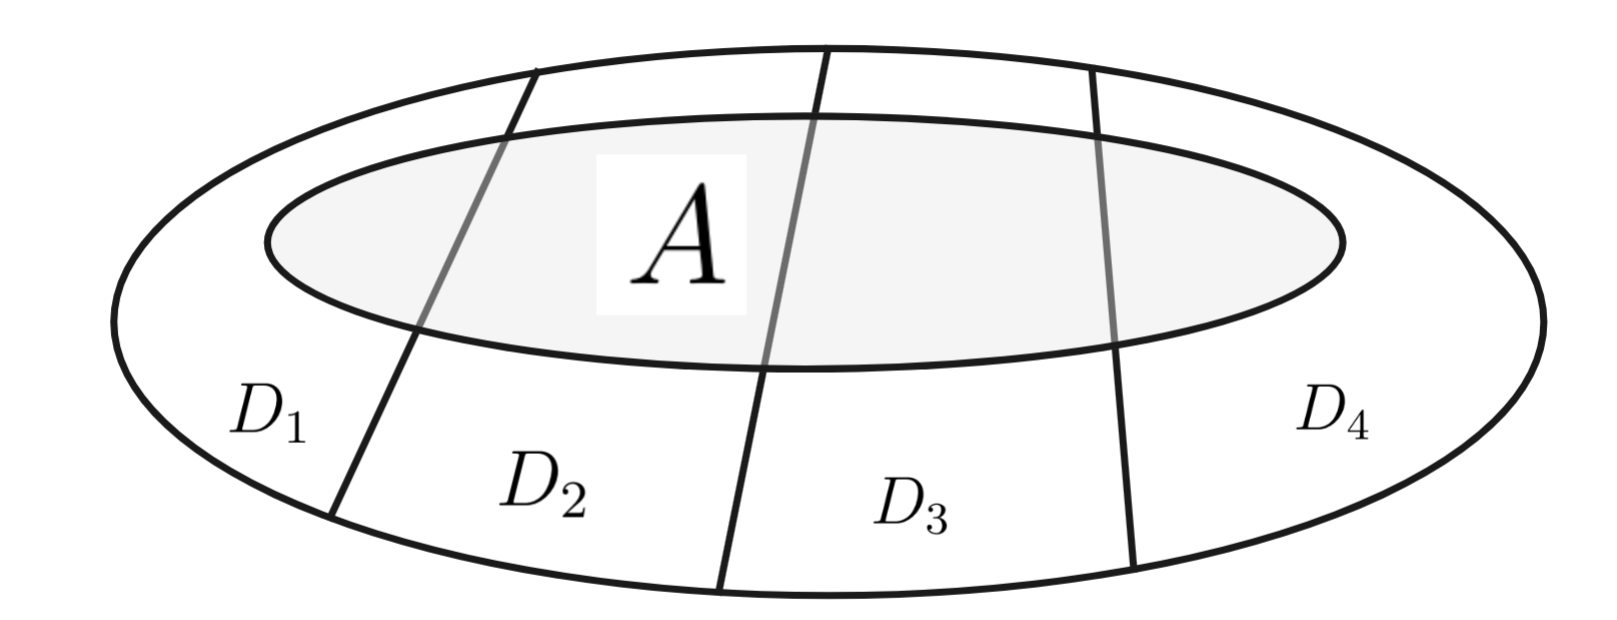
\includegraphics[width=0.6\textwidth ]{images/probTotale.png}
    }
\end{figure}
\subsubsection{Formula di Bayes}
Questo è il caso analogamente opposto a quello visto precedentemente, sia \(D_1,D_2,D_3...,D_k\)  una partizione 
di \(\Omega\), e sia \(A\subseteq \Omega\) un evento che 
segue uno degli eventi \(D_i\), sapendo che si è verificato \(A\), possiamo calcolare la probabilità che si 
sia verificato un singolo \(D_i\) : 
\begin{equation}
    \mathbb{P}(D_i|A)=\dfrac{ \mathbb{P}(D_i)\cdot \mathbb{P}(A|D_i)}{\displaystyle\sum_{j=1}^{k-1}\mathbb{P}(D_j)\cdot \mathbb{P}(A|D_j)}
\end{equation}
\textit{Osservazione} : Se \(A,B\) sono eventi disgiutni, allora \(\mathbb{P}(A|B)=\mathbb{P}(A)\).
\\\hphantom{}\\
Vediamo adesso un esempio facile di applicazione della formula delle probabilità totali, per ricavare 
il valore di una probabilità appartenente non banale. Si consideri lo schema di Bernoulli \ref{schemaBernoulli},
su \(n\) lanci, qual'è la probabilità che esca testa, un numero pari di volte? Voglio procedere \textit{ricorsivamente}
in \(n\), similmente a come si risolvono le equazioni di ricorrenza viste nel corso di \color{blue}\href{https://github.com/CasuFrost/University_notes/blob/main/Primo%20Anno/Secondo%20Semestre/Introduzione%20agli%20algoritmi/Introduzione_agli_Algoritmi.pdf}{Algoritmi 1}.
\color{black}\\Definisco \(A_n=\{\text{Su \(n\) lanci, testa esce un numero pari di volte}\}\) e \(p_n=\mathbb{P}(A_n)\). 
Procedo utilizzando la formula delle probabilità totali, definendo le partizioni : \begin{itemize}
    \item \(D_1=\{\omega \in \Omega | \omega_1=0\}\) - al primo lancio esce croce, ovviamente \(\mathbb{P}(D_1)=1-p\)
    \item \(D_2=\{\omega \in \Omega | \omega_1=1\}\) - al primo lancio esce testa, ovviamente \(\mathbb{P}(D_2)=p\)
\end{itemize}
Ed ottengo :\begin{equation}
    p_n= \mathbb{P}(D_1)\mathbb{P}(A_n|D_1)+\mathbb{P}(D_2)\mathbb{P}(A_n|D_2)
\end{equation}
Dove \(\mathbb{P}(A_n|D_1)\) rappresenta la probabilità che Su \(n-1\) lanci, testa esce un numero pari di volte, 
e \(\mathbb{P}(A_n|D_2)\) rappresenta la probabilità che Su \(n-1\) lanci, testa esce un numero dispari di volte. Quindi 
l'equazione si può riscrivere come : 
\begin{equation}
    p_n= (1-p)p_{n-1}+p(1-p_{n-1})
\end{equation}
Abbiamo definito una relazione \textit{ricorsiva}, che tramite passaggi algebrici può essere 
espressa in forma esplicita.
\subsubsection{Mappa sulla Probabilità Condizionata}
Quando si vuole calcolare la probabilità di un evento con la condizioni che un'altro evento si sia 
verificato, è possibili applicare la formula che abbiamo visto all'inizio di questo paragrafo. Un altra via 
da seguire però, può essere quella di considerare un \textbf{nuovo spazio di probabilità}, in cui si considerano come 
eventi elementari, esclusivamente quelli che già includono che la condizione si 
sia verificata.\\\hphantom{}\\ Se \(A\) è l'evento condizionante, posso considerare :
l'applicazione:\begin{center} \(B\subset\Omega,\text{ } B\rightarrow\mathbb{P}(B|A)\)\end{center} Ossia la mappa che ad ogni evento di \(\Omega\), associa 
la sua probabilità con condizione \(A\) verificata. Tale mappa, è ancora una funzione di probabilità, sullo 
spazio degli eventi \(A\), ciò è di facile dimostrazione:\begin{equation}
    \forall B\subset A,\text{ }\mathbb{P}(B|A)\in[0,1]
\end{equation}\begin{equation}
    \begin{cases}\mathbb{P}(\emptyset|A)=0\\
        \mathbb{P}(A|A)=\dfrac{\mathbb{P}(A\cap A)}{\mathbb{P}(A)}=\dfrac{\mathbb{P}(A)}{\mathbb{P}(A)}=1
       \end{cases} 
\end{equation}
Inoltre, tale funzione è additiva :
\begin{equation}
    B_1,B_2\subset A,\text{ }\mathbb{P}(B_1\cup B_2|A)=\mathbb{P}(B_1|A)+\mathbb{P}( B_2|A)
\end{equation}
\begin{center}\(
   \dfrac{\mathbb{P}((B_1\cup B_2)\cap A)}{\mathbb{P}(A)}=\dfrac{\mathbb{P}((B_1\cap A)\cup(B_2\cap A))}{\mathbb{P}(A)}\implies\text{per additività di \(\mathbb{P}\) }\implies
    \dfrac{\mathbb{P}(B_1\cap A)}{\mathbb{P}(A)}+\dfrac{\mathbb{P}(B_2\cap A)}{\mathbb{P}(A)}
\)\end{center}
\textbf{Osservazione 1 : }Se \(\mathbb{P}\) è la probabilità uniforme su \(\Omega\), preso l'evento 
fissato \(A\subset\Omega\), l'applicazione \(B\subset\Omega,\text{ } B\rightarrow\mathbb{P}(B|A)\) è 
anche essa ancora una probabilità uniforme.




\subsection{Passeggiata Aleatoria}
\subsubsection{La Rovina del Giocatore}
Introduciamo adesso un'altro problema meno banale rispetto a quello appena visto, che richiede sempre l'applicazione 
della formula delle probabilità totali. Ci sono due giocatori \(A\) e \(B\), che giocano ad un gioco generico, scomemttendo dei soldi. 
Ogni volta che un giocatore vince, riceve 1 euro dall'altro. \(A\) ha probabilità di vittoria uguale a \(p\), 
e \(B\) ha probabilità di vittoria uguale a \(1-p\), \(A\) inizia il gioco con un capitali pari ad \(a\) euro, 
e \(B\) inizia con un capitale pari a \(b\) euro. Giocano senza sosta, finche uno dei due giocatori 
non si rovina (finisce tutto il capitale). Qual'è la probabilità che \(A\) oppure \(B\) si rovini?
\subsubsection{Modellizzazione}
Tale problema ha un interpretazione geometrica ben precisa, e viene modellizzato in uno schema 
definito come \textit{passeggiata aleatoria}. Si consideri il piano \(\mathbb{Z}^+\times \mathbb{Z}\) : \\\begin{center}
    
    \includegraphics[scale=0.65]{images/PasseggiataAleatoriaPiano.eps}
\end{center}
l'asse 
delle ascisse \(t\) rappresenta il tempo, o il numero 
di giocate fatte, mentre quello delle ordinate \(S\) rappresenta la somma in denaro vinta da \(A\), ci sono poi 
due asintoti orizzontali nelle posizioni \(S=b\) e \(S=-a\).
Ad ogni coppia \(t,S\) è associato un valore denominato \(S_n\), che identifica l'istante di gioco, 
ossia la somma vinta (o persa se in negativo) da \(A\) al tempo \(t=n\). All'avanzare del tempo, ossia 
delle giocate, la crescita o discesa di \(S_n\) dipende dalle probabilità che \(A\) vinca o no, se 
\(A\) vince al tempo \(i\), nel tempo \(i+1\), \(S_n\) crescerà di un'unità, altrimenti decrescerà. \begin{itemize}
    \item \(t=0\implies S_0 = 0\)
    \item \(t=1 \implies S_1=\begin{cases}
        +1 \text{ con probabilità }p\\-1  \text{ con probabilità }1-p
    \end{cases}\)
    \item \(t=2 \implies S_2=S_1 +\begin{cases}
        +1 \text{ con probabilità }p\\-1  \text{ con probabilità }1-p
    \end{cases}\)
    \item \(...\)
    \item \(t=n+1\implies S_{n+1} = \displaystyle \sum_{i=1}^{n}S_i +\begin{cases}
        +1 \text{ con probabilità }p\\-1  \text{ con probabilità }1-p
    \end{cases}\)
\end{itemize}
Quindi nel grafico, \(S_n\) "spostandosi" verso destra, oscillerà avvicinandosi sempre di più o a
 \(b\) o a \(-a\), con ovvio significato :\begin{itemize}
    \item \(S_n=b\implies\) il giocatore \(B\) si è rovinato, ha vinto \(A\).
    \item \(S_n=-a\implies\) il giocatore \(A\) si è rovinato, ha vinto \(B\).
 \end{itemize}
 \begin{center}\includegraphics[scale=0.75]{images/PasseggiataRovinata.eps}\end{center}
 La probabilità che \(A\) si rovini è quindi equivalente alla probabilità che \(S_n\) raggiunga \(-a\), si può 
 calcolare tale valore utilizzando la formula delle probabilità totali.\\\hphantom{}\\
  Introduciamo un nuovo parametro, 
 ossia \(x\), che equivale ad \(S_0\), ossia quanto vale \(S\) all'inizio del gioco, fin'ora, abbiamo 
 dato per scontato che si partisse sempre da una condizione di parità, dove \(x=0\). Definiamo 
 quindi \(\alpha(x)\) la probabilità che \(S_n\) raggiunga \(-a\) da un punto di partenza \(x\), e  
 \(\beta(x)\) la probabilità che \(S_n\) raggiunga \(b\) da un punto di partenza \(x\). Ovviamente 
 se \(x=0\) siamo nel caso iniziale, ma ad ogni passo, \(x\) incrementerà o decrementerà di \(1\).
 Definiamo quindi \(S^{(x)}_n\) come la somma vinta da \(A\) nell'istante \(t=n\), dove però \(S^{(x)}_0\ne 0 = x\).
\\Vediamo come si definisce in questo caso una relazione ricorsiva, utilizzo la formula della 
probabilità totale :
\begin{equation}
    \beta(x)=\mathbb{P}(S_n+=1)\cdot\mathbb{P}(B \text{ si rovina }|S_n+=1)+\mathbb{P}(S_n-=1)\cdot\mathbb{P}(B \text{ si rovina }|S_n-=1)
\end{equation}
Ne consegue : \begin{equation}
    \beta(x)=p\cdot\beta(x+1)+(1-p)\cdot \beta(x-1) \text{ finché }x=-a\lor x=b
\end{equation}
Abbiamo quindi definito una relazione ricorsiva :\begin{center}
    \(
        \begin{cases}
            \beta(x)=p\cdot\beta(x+1)+(1-p)\cdot \beta(x-1)\\
            \beta(b)=1\\\beta(-a)=0
        \end{cases}
    \)
\end{center}
Sviluppiamo il calcolo per ottenere la formula esplicita, iniziando a calcolare l'incremento :
\begin{equation}
    (p+(1-p))\beta(x)=p\cdot\beta(x+1)+(1-p)\cdot \beta(x-1)\iff p(\beta(x+1)-\beta(x))=(1-p)(\beta(x)-\beta(x-1))
\end{equation}
\begin{equation}
    \iff \beta(x+1)-\beta(x)=\dfrac{1-p}{p}(\beta(x)-\beta(x-1))
\end{equation}
Gli incrementi sono quindi \textit{proporzionali} e non lineari (simile alla funzione esponenziale).
Avendo trovato adesso il valore ad ogni incremento generico, procediamo calcolando l'incremento ad ogni passo :
\begin{itemize}
    \item passo 0) \(\beta(-a)=0\)
    \item passo 1)  \(\beta(-a+1)=\beta(-a+1)-\beta(-a)=\beta(-a+1)-0=\gamma\) 
\end{itemize}
Abbiamo definito \(\gamma\) come l'incremento ad ogni passo \begin{itemize}
    \item passo 2) \(\beta(-a+2) =\beta(-a+1)+\beta(-a+2)-\beta(-a+1)+\dfrac{1-p}{p}\gamma=\gamma+\gamma\dfrac{1-p}{p} \)
    \item passo 3) \(\beta(-a+3)=\beta(-a+2)+\beta(-a+3)-\beta(-a+2)=\beta(-a+2)+\dfrac{1-p}{p}[\beta(-a+2)-\beta(-a+1)]=\)\\
    \(\gamma+\gamma\dfrac{1-p}{p}+\gamma(\dfrac{1-p}{p})^2\)
    \item \dots
    \item \(\beta(x)=\gamma\Big[1+\dfrac{1-p}{p}+\Big(\dfrac{1-p}{p}\Big)^2+\Big(\dfrac{1-p}{p}\Big)^3...+\Big(\dfrac{1-p}{p}\Big)^{x+a-1}\Big]\)
\end{itemize}
Quindi si ha che \begin{equation}
    \beta(x)=\gamma\cdot \sum_{k=0}^{x+a-1}\Big(\dfrac{1-p}{p}\Big)^k=\gamma\cdot\dfrac{1-\Big(\dfrac{1-p}{p}\Big)^{x+a}}{1-\dfrac{1-p}{p}}
\end{equation}
Per trovare \(\gamma\), poniamo :
\begin{equation}
    \beta(b)=1=\gamma\cdot\dfrac{1-\Big(\dfrac{1-p}{p}\Big)^{b+a}}{1-\dfrac{1-p}{p}}\implies \gamma =\dfrac{1-\dfrac{1-p}{p}}{1-\Big(\dfrac{1-p}{p}\Big)^{b+a}}
\end{equation}
Quindi, in forma esplicita :\begin{equation}
    \beta(x)=\dfrac{1-\Big(\dfrac{1-p}{p}\Big)^{x+a}}{1-\Big(\dfrac{1-p}{p}\Big)^{b+a}}
\end{equation}
\textit{Osservazione }: la probabilità che il gioco non finisca mai è 0, infatti presi i due eventi della rovina 
di \(A\) e di \(B\), si ha che :\begin{equation}
    \alpha(a)+\beta(b)=\dfrac{1-\Big(\dfrac{1-p}{p}\Big)^{x+b}}{1-\Big(\dfrac{1-p}{p}\Big)^{b+a}}+\dfrac{1-\Big(\dfrac{1-p}{p}\Big)^{x+a}}{1-\Big(\dfrac{1-p}{p}\Big)^{b+a}}=1
\end{equation}
La somma dei due eventi disgiunti è 1, quindi, necessariamente si causerà la rovina di uno dei due giocatori.
\\\textit{Osservazione }: Se \(p=\dfrac{1}{2}\), si ha :
\begin{equation}
    \lim_{p\rightarrow \frac{1}{2}}\beta(x)=\lim_{p\rightarrow \frac{1}{2}}\dfrac{1-\Big(\dfrac{1-p}{p}\Big)^{x+a}}{1-\Big(\dfrac{1-p}{p}\Big)^{b+a}}=\dfrac{a+x}{a+b}
\end{equation}
\textit{Esempio }: Se \(A\) parte da 5 euro, ed ha probabilità di vittoria uguali a 0.4, e 
\(B\) parte da 7 euro, ed ha probabilità di vittoria uguali a 0.6, si ha che :\begin{itemize}
    \item La probabilità che \(B\) si rovini è : \(\dfrac{1-\Big(\dfrac{1-0.4}{0.4}\Big)^{5}}{1-\Big(\dfrac{1-0.4}{0.4}\Big)^{5+7}}\simeq  0,05\)
\end{itemize}\newpage
\section{Variabili Aleatorie}
Dato uno schema probabilistico \((\Omega,\mathbb{P})\), una \textbf{variabile aleatoria} \(X\) è una 
funzione su \(\Omega\) a valori reali:\begin{center}
    \(X:\Omega\rightarrow\mathbb{R}\)
\end{center}
Tale variabile, rappresenta una "scommessa" sull'esito di un esperimento, ad ogni evento elementare o insieme 
di eventi elementari, è associato un valore reale.\\\textit{Esempio :} Si lancia un dado equo, e ci sono 2 
giocatori, \(A\) e \(B\). Se il dado da come esito 1 o 2, il giocatore \(A\) paga 2 euro, se da come 
esito 3, il giocatore \(A\) paga 1 euro, se da come esito 4, il giocatore \(B\) paga 1 euro, se da come 
esito 5 o 6, il giocatore \(B\) paga 2 euro, tale "pagamento" è esprimibile come variabile aleatoria, dove il suo 
valore rappresenta la quota vinta o persa da \(A\) :\begin{center}
    \(X_1=
    \begin{cases}
        -2\text{ se }\omega=1,2\\
        -1\text{ se  }\omega=3\\
        1\text{  se }\omega=4\\
        2\text{ se  }\omega=5,6
    \end{cases}    
    \)
\end{center}
In questo caso, \(X_1\) non è iniettiva, se lo fosse però, in base al risultato della scommessa, sarebbe possibile 
conoscere l'esito del dado ( in questo caso, se \(A\) paga 2 euro, non sappiamo se il dado abbia dato come esito 1 o 2).
 \\ Una variabile aleatoria \(X\) può essere rappresentata come un \textit{istogramma}, dove sull'asse delle 
 ascisse è presente l'immagine di \(X\), e sulle ordinate la probabilità che ogni valore di \(X\) si verifichi.
 Per l'esempio preso in considerazione prima :
 \\\begin{center}
    \includegraphics[scale=1.5]{images/istogramma.eps}
\end{center}
La probabilità \(\mathbb{P}\) su \(\Omega\), \textit{induce} una probabilità sull'immagine 
della variabile aleatoria, denominata \(Im(X)\), mediante la funzione \(\Im\) :
\begin{center}
    Sia \(x_1\in Im(X)\), \(\Im(\{x_1\}):=\mathbb{P}(\{\omega\in\Omega|X(\omega)=x_1\})\)
\end{center}
Rappresenta la probabilità che \(X\) assuma un certo valore \(x_1\), definisce la \textbf{distribuzione}
della variabile aleatoria.
\\\textit{Notazione} :\(\Im(\{x_1\})\) può essere scritto anche come \(\Prob(X=x_1)\)
\subsection{Valore Atteso}
Il \textbf{valore atteso} di una variabile aleatoria \(X\) è una funzione \(\mathbb{E}\) definita nel seguente modo :\begin{center}
   \( \mathbb{E}(X)=\displaystyle\sum_{x\in Im(x)}x\cdot \Im(\{x\})\)
\end{center}
È dato dalla somma dei possibili valori di tale variabile,
ciascuno moltiplicato per la probabilità di essere assunto (ossia di verificarsi).\\
Indica il valore medio che \(X\) può assumere, a seconda delle probabilità di ogni valore dell'immagine di \(X\).
\\\hphantom{}\\\textit{Esempio :} Si lancia un dado, ci sono due giocatori \(A\) e \(B\), la variabile aleatoria \(X\) 
rappresenta la quota in euro vinta da \(A\) in base all'esito del dado (se negativa, è la quota che \(A\) deve pagare 
a \(B\)).\begin{center}
    \(
    X=\begin{cases}
        -1\text{ se }\omega=1,2\\
        0\text{ se  }\omega=3\\
        1\text{  se }\omega=4\\
        2\text{ se  }\omega=5,6
    \end{cases}    
    \)
\end{center}
In questo gioco è ovvio che \(A\) sia avvantaggiato, dato che in soli 2 esiti su 6 dovrà pagare. 
In base a questo schema, \(A\) sicuramente si troverà a vincere più denaro di \(B\), ma quanto precisamente?
Tale quota, è data dal valore atteso :\begin{center}
    \(
    \mathbb{E}(X)=(-1)\cdot\dfrac{2}{6}+0\cdot\dfrac{1}{6}+1\cdot\dfrac{1}{6}+2\cdot\dfrac{2}{6} =0.5   
    \)
\end{center}
Quindi, deduciamo che per rendere il gioco equo, \(A\) prima di ogni lancio, dovrebbe 
dare a \(B\) 0.5 euro.
\\\hphantom{}\\Una possibile rappresentazione "fisica" che si può dare al valore, atteso è la seguente :\\
Si consideri l'istogramma di una variabile aleatoria, si immagini l'asse delle ascisse come un asse 
privo di massa che si appoggia su un perno, e i valori dell'immagine della variabile, come delle colonne 
che hanno massa uguale alla loro probabilità, il valore atteso non è altro che, la posizione in cui si deve trovare 
il perno per far si che l'asse sia in equilibrio, per l'esempio precedente :\begin{center}
    \includegraphics[scale=1.5]{images/istogrammaFisico.eps}
\end{center}
\subsubsection{Linearità del Valore Atteso}\label{linE}
Se \(\Omega\) è un insieme finito, e \(\mathcal{V}\) l'insieme delle sue variabili aleatorie, ossia 
tutte le funzioni \(X:\Omega\rightarrow\mathbb{R}\), \(\mathcal{V}\) assume una naturale struttura 
di \textit{spazio vettoriale}.\begin{itemize}
    \item \(\alpha\in\mathbb{R}\) ed \(X\in\mathcal{V}\) si ha \((\alpha \cdot  X)(\omega)=\alpha\cdot X(\omega)\)\hphantom{text} \(\forall \omega\in\Omega\)
    \item \(X,Y\in\mathcal{V}\) si ha \((X+Y)(\omega)=X(\omega)+Y(\omega)\)\hphantom{t-ext} \(\forall \omega\in\Omega\)
\end{itemize}
Effettivamente, se \(|\Omega|=n\), c'è un isomorfismo canonico fra \(\mathcal{V}\) ed \(\mathbb{R}^n\).\\
Il valore atteso, definito come \(\mathbb{E}:\mathcal{V}\rightarrow\mathbb{R}\) è un \textbf{applicazione lineare} :
\begin{equation}\forall \alpha\in\mathbb{R}\text{, }\forall X,Y\in \mathcal{V} :
    \begin{cases}
        \mathbb{E}(\alpha \cdot X)=\alpha\cdot \mathbb{E}(X)\\
        \mathbb{E}(X+Y)=\mathbb{E}(X)+\mathbb{E}(Y)
    \end{cases}
\end{equation}
\textbf{Dimostrazione }: Si consideri la seguente osservazione preliminare :\begin{center}
    \(
    \E(X)=\displaystyle\sum_{\omega\in\Omega}X(\omega)\cdot\Prob(\{\omega\})
    =\sum_{\omega\in\Omega|X(\omega)=x}\Prob(\{\omega\})\cdot\sum_{x\in Im(X)}x=
    \displaystyle\sum_{x\in Im(x)}x\cdot \Im(\{x\})
    \)
\end{center}
Con la nuova definizione alternativa di valore atteso 
\(
    \E(X)=\displaystyle\sum_{\omega\in\Omega}X(\omega)\cdot\Prob(\{\omega\})
    \)
Posso dimostrare la linearità di esso :\begin{equation}
    \E(\alpha X)=\sum_{\omega\in\Omega}(\alpha X)(\omega)\cdot\Prob(\{\omega\})=\sum_{\omega\in\Omega}\alpha\cdot X(\omega)\cdot\Prob(\{\omega\})=\alpha\E(X)
\end{equation}\begin{equation}
    \E(X+Y)=\sum_{\omega\in\Omega}(X+Y)(\omega)\cdot\Prob(\{\omega\})=\sum_{\omega\in\Omega}(X(\omega)+Y(\omega))\cdot\Prob(\{\omega\})=\E(X)+\E(Y)
\end{equation}
\raggedleft\(\blacksquare\)\\
\raggedright

\subsection{Varianza}
Introduciamo un altro valore associato alle variabili aleatorie.\\
La \textbf{varianza} di una variabile aleatoria è una funzione \(\mathbb{V}\) strettamente maggiore di 0, definita nel seguente modo :
\begin{center}
    \(
    \mathbb{V}(X)=\displaystyle\sum_{x\in Im(X)}(x-\mathbb{E}(X))^2\cdot   \Im(\{x\})  
    \)
\end{center}
È lo scarto quadratico medio, ossia, una misura di quanto i valori si discostino 
quadraticamente rispetto al valore atteso. Una varianza piccola, indica che la variabile 
aleatoria è \textit{distribuita} vicino il valore medio.\\\hphantom{}\\
Si consideri l'esempio visto in precedenza : si lancia un dado, ci sono due giocatori \(A\) e \(B\), la variabile aleatoria \(X\) 
rappresenta la quota in euro vinta da \(A\) in base all'esito del dado (se negativa, è la quota che \(A\) deve pagare 
a \(B\)).\begin{center}
    \(
    X_1=\begin{cases}
        -1\text{ se }\omega=1,2\\
        0\text{ se  }\omega=3\\
        1\text{  se }\omega=4\\
        2\text{ se  }\omega=5,6
    \end{cases}    
    \)
\end{center}
In questo caso la varianza rappresenta il rischio che si corre, dato che, se la possibile perdita fosse molto 
alta, la varianza risulterebbe a sua volta elevata. In questo caso si ha :
\begin{equation}
    \mathbb{V}(X_1)=(-1-0.5)^2\cdot \dfrac{2}{6}+(0-0.5)^2\cdot \dfrac{1}{6}+(1-0.5)^2\cdot \dfrac{1}{6}+(2-0.5)^2\cdot \dfrac{2}{6}\simeq1,58
\end{equation}
De facto, la varianza non è elevata, in quanto il rischio di perdita, rispetto a quello di vincita, non rappresenta una grande differenza di denaro,
se dovessi infatti cambiare il denaro perso si avrebbe :
\begin{center}
    \(
    X_2=\begin{cases}
        -50\text{ se }\omega=1,2\\
        0\text{ se  }\omega=3\\
        1\text{  se }\omega=4\\
        2\text{ se  }\omega=5,6
    \end{cases}    
    \)
\end{center}
\begin{equation}
    \mathbb{V}(X_2)=(-50-0.5)^2\cdot \dfrac{2}{6}+(0-0.5)^2\cdot \dfrac{1}{6}+(1-0.5)^2\cdot \dfrac{1}{6}+(2-0.5)^2\cdot \dfrac{2}{6}\simeq850
\end{equation}
\subsection{Variabili Aleatorie Note}
In questo paragrafo vedremo i casi più comuni di variabili aleatorie.
\subsubsection{Variabile Aleatoria Certa}
Questo è il caso in cui la variabile aleatoria \(X\) è una funzione costante:\begin{center}
   \(\exists\tilde x\in \mathbb{R}|X(\omega)=\tilde x \forall \omega\in \Omega\) quindi \(|Im(X)|=1\)
\end{center}
Ovviamente, la varianza risulta nulla : \(\mathbb{V}(X)=0\).
\subsubsection{Variabile Aleatoria di Bernoulli}
Sia \(p\in[0,1]\) una costante reale, e \(X\) una variabile aleatoria che ha solamente due 
valori nell'immagine : \(Im(X)=\{a,b\}\), dove \(\Im(\{a\})=p\) e \(\Im(\{b\})=1-p\).
Dove rispettivamente \(a=1\) e \(b=0\).
\begin{center}
    \includegraphics[scale=1]{images/VABernoulli.eps}
\end{center}
In questo caso varianza e valore atteso valgono : \begin{equation}
    \mathbb{E}(X)=0\cdot(1-p)+1\cdot p = p
\end{equation}\begin{equation}
    \mathbb{V}(X)=(0-p)^2(1-p)+(1-p)^2p=p(1-p)(p+1-p)=p(1-p)
\end{equation}
Se \(p=\dfrac{1}{2}\), la varianza è massima.
\subsubsection{Variabile Aleatoria Binomiale}
Considerando lo schema di Bernoulli : \(\Omega=\{0,1\}^n\), dove \(p\) è la probabilità che \(\omega_i\) assuma 
valore \(1\), la variabile aleatoria binomiale \(X\) conta 
il numero di \(1\), ossia \(X(\omega)=\displaystyle \sum_{i=1}^n\omega_i\). \\Ad esempio, per \(n=2\) si ha : 
\begin{center}
    \(
    X=\begin{cases}
        0\text{ se }\omega=00\\
        1\text{ se  }\omega=01\\
        1\text{  se }\omega=10\\
        2\text{ se  }\omega=11
    \end{cases}    
    \)
\end{center}
Abbiamo già visto in precedenza qual'è la probabilità che il numero di 1 sia \(k\) :\begin{center} 
    \(\Im(\{k\})=\displaystyle \binom{n}{k}p^k(1-p)^{n-k}\)\end{center}
    Il valore di attesa vale :
    \begin{equation}
        \mathbb{E}(X)=\sum_{k=0}^nk\cdot \Im(\{k\})=\sum_{k=0}^nk\binom{n}{k}p^k(1-p)^{n-k}=n\cdot p
    \end{equation}
Possiamo sfruttare la \textit{linearità} del valore atteso \ref{linE} per calcolare il valore atteso 
della variabile aleatoria binomiale senza calcoli complessi.
Consideriamo \(X_i\) la variabile aleatoria definita nel seguente modo : \begin{equation}
    X_i=\begin{cases}
        1 \text{ se l'}i\text{-esimo lancio ha fatto testa}\\
        0 \text{ se l'}i\text{-esimo lancio ha fatto croce}\\
    \end{cases}
\end{equation}
Per cui risulta \(\E(X_i)=p\), da qui osservo che :\begin{equation}
    \E(X)=\sum_{i=1}^n\E(X_i)=\sum_{i=1}^np=n\cdot p
\end{equation}
Calcoliamo adesso la varianza della variabile aleatoria di Bernoulli, ma prima facciamo un'osservazione, in generale
è vero che  :\begin{center}
    \(\V(X)=\E(X^2)-(\E(X))^2\)
\end{center}
Dimostrazione :\begin{center}\(
    \V(X)=\displaystyle\sum_{x\in Im(X)}(x-\mathbb{E}(X))^2\cdot\Im(\{x\})  =\E(X-\E(X)^2)=\E(X^2-2X\E(X)+\E(X)^2)
\)\\\(
    =\E(X^2)-2\E(X\E(X))+\E(\E(X)^2)=\E(X^2)-2\E(X)\E(X)+\E(\E(X)^2)=\E(X^2)-(\E(X))^2\) \(\blacksquare\)
\end{center}
Quindi calcoliamo il valore di \(\E(X^2)\) per la variabile aleatoria di bernoulli :
\begin{equation}
    \E(X^2)=\sum_{k=0}^nk^2\Prob(X=k)=\sum_{k=1}^nk\dfrac{n!}{(k-1)!(n-k)!}p^k(1-p)^{n-k}
\end{equation}
\begin{equation}
    =\sum_{k=1}^n1\dfrac{n!}{(k-1)!(n-k)!}p^k(1-p)^{n-k}+\sum_{k=2}^{n-1}(k-1)\dfrac{n!}{(k-2)!(n-k)!}p^k(1-p)^{n-k}
\end{equation}\begin{equation}
    =np+\sum_{k=2}^n\dfrac{n(n-1)(n-2)!}{(k-2)!(n-k)!}p^k(1-p)^{n-k}
\end{equation}
Sostituisco \(h=k-2\) : \begin{equation}
    np+n(n-1)\sum_{k=2}^n\dfrac{n(n-1)(n-2)!}{(h-2)!(n-h-2)!}p^h(1-p)^{n-h-2}=np+n(n-1)\binom{n-2}{h}p^h(1-p)^{n-h-2}
\end{equation}
\begin{equation}
    =np+n(n-1)p^2
\end{equation}
Quindi :\begin{equation}
    \V(X)=\E(X^2)+(\E(X))^2=np+n(n-1)p^2+(np)^2=np(1-p)
\end{equation}
Considerando \begin{equation}
    X_i=\begin{cases}
        1 \text{ se l'}i\text{-esimo lancio ha fatto testa}\\
        0 \text{ se l'}i\text{-esimo lancio ha fatto croce}\\
    \end{cases}
\end{equation}
Si nota che \(\V(X)=\displaystyle\sum_{i=1}^n\V(X_i)\), sembrerebbe quindi che la varianza sia lineare, ma ciò 
è falso, dato che la varianza presenta uno scarto quadratico. Il fatto è che ciò è vero per la variabile
aleatoria di bernoulli, perché le diverse \(X_i\) fra loro sono \textit{indipendenti}.
\subsection{Variabili Aleatorie Indipendenti}
Siano \(X,Y\in\mathcal{V}\) due variabili aleatorie, se \(\forall x\in Im(X)\) e \(\forall y\in Im(Y)\) vale che :
\begin{center}
    \(
      \Prob(\{X=x\}\cap\{Y=y\})=\Prob(X=x)\cdot\Prob(Y=y)  
    \)
\end{center}
Le due variabili aleatorie si dicono \textbf{indipendenti}.\\\hphantom{}\\
\textbf{Proposizione} : Se \(X\) ed \(Y\) sono indipendenti, vale la seguente identità :\begin{center}
    \(\V(X+Y)=\V(X)+\V(Y)\)
\end{center}
Detto ciò, risulta chiaro del perché, per \(X=\)\{Variabile Aleatoria di Bernoilli\}, si ha che \(\V(X)=np(1-p)\).
Vediamo adesso, dimostriamo la \textit{proposizione}.\\\hphantom{}\\
\textbf{Dimostrazione della proposizione} : Sviluppo la varianza della somma :
\begin{equation}
    \V(X+Y)=\E([X+Y-\E(X+Y)]^2)=\E([X-\E(X)+Y-\E(Y)]^2)
\end{equation}
\begin{equation}
    = \E((X-\E(X))^2+(Y-\E(Y))^2+2((X-\E(X))(Y-\E(Y))))
\end{equation}
\begin{equation}
    =\V(X)+\V(Y)+2\E((X-\E(X))(Y-\E(Y)))
\end{equation}
Il termine \(\E((X-\E(X))(Y-\E(Y)))\) è detto \textit{covarianza}, bisogna dimostrare che la covarianza è 
nulla se \(X\) ed \(Y\) sono indipendenti.\\\hphantom{}\\
\textbf{Osservazione} : Se la covarianza è nulla, allora \(\E(X\cdot Y)=\E(X)\cdot\E(Y)\), questo perché :\begin{equation}
    \E((X-\E(X))(Y-\E(Y)))=\E(X)\E(Y)-\E(X)\E(Y)+\E(X)\E(Y)=\E(X\cdot Y)=\E(X)\cdot\E(Y) 
\end{equation}
Quindi bisogna dimostrare che, se \(X,Y\) sono indipendenti, \(\E(X\cdot Y)=\E(X)\cdot\E(Y) \).
\\\textit{Passo finale della dimostrazione} : \begin{equation}
    \E(X\cdot Y)=\sum_{\omega\in \Omega}X(\omega)Y(\omega)\Prob({\omega})=
    \sum_{x\in Im(X)}x\cdot\sum_{y\in Im(Y)}y\cdot\sum_{
        \omega\in\Omega|X(\omega)=x\land Y(\omega)=y
    }\Prob(\{X=x\}\cap\{Y=y\})
\end{equation}
Per indipendenza :  \(
    \Prob(\{X=x\}\cap\{Y=y\})=\Prob(X=x)\cdot\Prob(Y=y)  
  \)
  Riscrivo :
  \begin{equation}
    \sum_{x\in Im(X)}x\Prob(X=x)\cdot\sum_{y\in Im(Y)}y\Prob(Y=y)=\E(X)\cdot\E(Y)\text{\hphantom{aaaa}}\blacksquare
  \end{equation}
  \subsubsection{La Covarianza}
  Diamo adesso una definizione ed un significato intrenseco alla \textbf{covarianza}
citata in precedenza. La covarianza è un valore associato a due variabili 
aleatorie ed è definita in tal modo :\begin{center}
    \(
    \text{Cov}(X,Y)=(X-\E(X))(Y-\E(Y))    
    \)
\end{center}
Euristicamente parlando, la covarianza misura la relazione di dipendenza di 
due variabili aleatorie, può essere positiva o negativa, se 
\(\text{Cov}(X,Y)\) è particolarmente grande, ciò significa che, 
sapere che \(X\) sia grande rende più probabile il fatto che \(Y\) 
sia grande, in generale la covarianza è limitata : \(|\text{Cov}(X,Y)|\le\sqrt{\V(X)}\cdot\sqrt{\V(Y)}\).
\acc 
\textit{Esempio} : Eseguo una misurazione su un circuito, \(X\) rappresenta 
la differenza di potenziale, ed \(Y\) l'intensità di corrente, la misurazione, avviene 
con una precisione tale, da poter osservare gli effetti aleatori, dovuti a fattori 
da noi non controllabili, per cui, nonostante la differenza di potenziale sia costante, 
diverse misurazioni differiscono nei valori decimali. Eseguo precisamente 
\(n\) misurazioni, e rappresento su un piano cartesiano il risultato, 
in cui \(\E(X)\) è l'asse delle ascisse, ed \(\E(Y)\) quello 
delle ordinate.
\begin{figure}[h]
    \centering{
    \includegraphics[width=0.75\textwidth ]{images/cov.eps}
    }
\end{figure}
\end{document}
